\documentclass[letterpaper]{article}
\usepackage[top=2cm, bottom=3.5cm, left=2.5cm, right=2.5cm]{geometry}
\usepackage{amsmath,amsthm,amssymb}
% Indicator function
\usepackage{bbm}
\usepackage{tikz}
\usepackage{enumitem}
\usepackage{booktabs}
\usepackage[T1]{fontenc}
\usepackage{indentfirst}

\usepackage{graphicx}
\usepackage{epstopdf}

% Bold vectors and matrices
\renewcommand{\aa}{\mathbf{a}}
\providecommand{\xx}{\mathbf{x}}
\providecommand{\yy}{\mathbf{y}}
\providecommand{\1}{\mathbf{1}}
\providecommand{\0}{\mathbf{0}}
\providecommand{\mA}{\mathbf{A}}
\providecommand{\mI}{\mathbf{I}}

\providecommand{\lin}[1]{\ensuremath{\left\langle #1 \right\rangle}}
\providecommand{\norm}[1]{\ensuremath{\left\lVert#1\right\rVert}}

%
% The following macro is used to generate the header.
%
\newcommand{\homework}[4]{
   \thispagestyle{plain}
   \newpage
   \noindent
   \begin{center}
   \framebox{
      \vbox{\vspace{2mm}
    \hbox to 6.28in { {\bf EE-556: Mathematics of Data \hfill Fall 2019} }
       \vspace{6mm}
       \hbox to 6.28in { {\Large \hfill Homework \##1 - Due date: #2\hfill} }
       \vspace{4mm}
       \hbox to 6.28in { {\hfill Student: #3} }
      \vspace{2mm}}
   }
   \end{center}
}

\renewcommand{\phi}{\varphi}
\renewcommand{\epsilon}{\varepsilon}

% Use these for theorems, lemmas, proofs, etc.
\newtheorem{proposition}{Proposition}
\newtheorem{theorem}{Theorem}
\newtheorem{corollary}{Corollary}
\newtheorem{lemma}{Lemma}
\newtheorem{claim}{Claim}
\newtheorem{remark}{Remark}
\newtheorem{definition}{Definition}
\newtheorem{fact}{Fact}
\newtheorem{assumption}{Assumption}

\DeclareMathOperator*{\argmin}{arg\,min}
\DeclareMathOperator*{\argmax}{arg\,max}
\newcommand{\mbeq}{\overset{!}{=}}
\newcommand{\E}{\mathbb{E}}
\newcommand{\vect}[1]{\boldsymbol{#1}}

% Use Small capitals like in problem statement
\usepackage{sectsty}
\renewcommand{\thesection}{\Roman{section}} 
\renewcommand{\thesubsection}{\Roman{subsection}}
\allsectionsfont{\mdseries\scshape}

\begin{document}
\homework{1}{1\textsuperscript{st} November 2019}{Oriol Barbany Mayor}

\subsection*{Problem 1 - Geometric properties of the objective function $f$}
\begin{enumerate}[label=(\alph*)]
    \item By linearity of the gradient operator, we have that
    \begin{align}
        f(\xx, \mu) := \frac{1}{n}\sum_{i=1}^n g_i (\xx, \mu) + \frac{\lambda}{2}\norm{\xx}^2 \Longrightarrow \nabla f(\xx) = \frac{1}{n}\sum_{i=1}^n \nabla g_i (\xx, \mu) + \lambda \xx
    \end{align}
    
    \begin{align}
        \nabla g_i (\xx, \mu) = \begin{cases}
        -b_i \aa_i, & b_i \aa_i^T \xx \leq 0\\
        b_i \aa _i (b_i \aa_i^T \xx - 1), &0<b_i\aa_i^T \xx \leq 1 \\
        0,& 1\leq b_i \aa_i^T \xx
        \end{cases}
        \label{eq:1}
    \end{align}
    which yields
    
    \begin{align}
        \nabla f(\xx) = \frac{1}{n}\sum_{i=1}^n \left[ -b_i \aa_i\mathbbm{1}_{\{b_i \aa_i^T \xx  \leq 0\}} + b_i\aa _i (b_i\aa_i^T \xx -1 )\mathbbm{1}_{\{0<b_i \aa_i^T \xx\leq 1\}} \right] + \lambda \xx
        \label{eq:2}
    \end{align}
    
    Note that with the proposed notation, $\mI_L$ selects the coordinates that are in the linear region (first case of \eqref{eq:1}), and $\mI_Q$ the ones that lie in the quadratic region (second case). If we express \eqref{eq:2} in matrix form using $\tilde{\mA}$ as given in the problem description and the previous matrices, we get
    \begin{align}
        \nabla f(\xx) = - \frac{1}{n} \tilde{\mA} \mI_L \1 + \frac{1}{n} \tilde{\mA}^T \mI_Q [\tilde{\mA} \xx - \1] + \lambda \xx
    \end{align}
    
    Let's now compute the Lipschitz constant of the gradient:
    \begin{align}
        \norm{\nabla f(\xx) - \nabla f(\yy)} &= \norm{\lambda (\xx - \yy) + \frac{1}{n}\tilde{\mA}^T \mI_Q\tilde{\mA} (\xx - \yy) - \frac{1}{n} \tilde{\mA} \mI_L \1 + \frac{1}{n} \tilde{\mA} \mI_L \1} \\
        &= \norm{\left( \lambda\mathbf{I} + \frac{1}{n}\tilde{\mA}^T \mI_Q\tilde{\mA} \right) (\xx - \yy)} \\
        &\leq \norm{\lambda\mathbf{I} + \frac{1}{n}\tilde{\mA}^T \mI_Q \tilde{\mA}} \norm{\xx - \yy}
    \end{align}
    where the inequality follows from definition of the spectral norm.
    
    Using the fact that $\lambda\mathbf{I} + \frac{1}{n}\tilde{\mA}^T \mI_Q \tilde{\mA} = \lambda\mathbf{I} + \frac{1}{n}\tilde{\mA}^T \tilde{\mA}$ given in the problem statement and using the triangle inequality, we get that
    \begin{align}
        \norm{\lambda\mathbf{I} + \frac{1}{n}\tilde{\mA}^T \mI_Q \tilde{\mA}} &=\norm{\lambda\mathbf{I} + \frac{1}{n}\tilde{\mA}^T \tilde{\mA}} := \max_{\xx:\norm{\xx}=1} \norm{\left( \lambda\mathbf{I} + \frac{1}{n}\tilde{\mA}^T \tilde{\mA} \right) \xx} \\
        &\leq |\lambda| \max_{\xx:\norm{\xx}=1} \norm{\xx}  +\frac{1}{n} \max_{\xx:\norm{\xx}=1}  \norm{\tilde{\mA}^T \tilde{\mA}\xx}
        := \lambda + \frac{1}{n}\norm{\tilde{\mA}^T \tilde{\mA}} \\
        &\leq \lambda + \frac{1}{n}\norm{\tilde{\mA}^T} \norm{\tilde{\mA}}
    \end{align}
    where the last inequality again follows from definition of the spectral norm and I assume that $\lambda$ is non-negative. The proof is completed using the fact that $\norm{\tilde{\mA}}=\norm{\mA}$ and $\norm{\tilde{\mA}^T}=\norm{\mA^T}$.
    
    \item Assuming that all the samples lie in the quadratic region, i.e. $\mI_Q = \mathbb{I}$ and $\mI_L=\0$:
    \begin{align}
        \nabla f(\xx) = \frac{1}{n} \tilde{\mA}^T [\tilde{\mA} \xx - \1] + \lambda \xx
    \end{align}
    
    The gradient $\nabla f$ exists in all domain of $\xx$ and correspond to a linear function on $\xx$, which is infinitely differentiable. We then say that $f$ is twice differentiable (in also fact infinitely differentiable and thus twice), and its hessian corresponds to
    \begin{align}
        \nabla^2 f(\xx) = \frac{1}{n} \tilde{\mA}^T \tilde{\mA} + \lambda\mathbb{I}=\frac{1}{n}\mA^T \mA + \lambda\mathbb{I}
    \end{align}
    where the equality follows since $b_i^2 = 1 \ \forall i$, which implies that $\tilde{\mA}^T \tilde{\mA} = \mA^T \mA$.
    
    \item 
    \begin{lemma}
        A function $f$ is $\mu-$strongly convex iff $\nabla^2 f(\xx) \succeq \mu \mathbb{I}$
        \label{prop:1}
    \end{lemma}
    \begin{proof}
        As seen in lectures, $f$ is $\mu-$strongly convex iff $g(\xx):=f(\xx)-\frac{\lambda}{2}\norm{\xx}$ is convex, and hence if $\nabla^2g(\xx) \succeq 0$. The proposition follows by combining these two.
    \end{proof}
    
    Given that we have the hessian of $f$, we can use Lemma \ref{prop:1} to compute the strong convexity constant:
    \begin{align}
        \xx^T \nabla^2 f(\xx) \xx  = \lambda + \frac{1}{n}\xx^T\mA^T \mA \xx \geq \lambda := \mu \quad \forall \xx
    \end{align}
    where the inequality follows since $\mA^T \mA$ is positive semidefinite. This latter is true since we can define $\yy:=\mA \xx$ and $\norm{y} := \yy^T \yy := \xx^T\mA^T \mA \xx $ will be non-negative by definition of the norm.
\end{enumerate}

\subsection*{Problem 2 - First order methods for SVM}
\begin{figure}[ht]
    \centering
    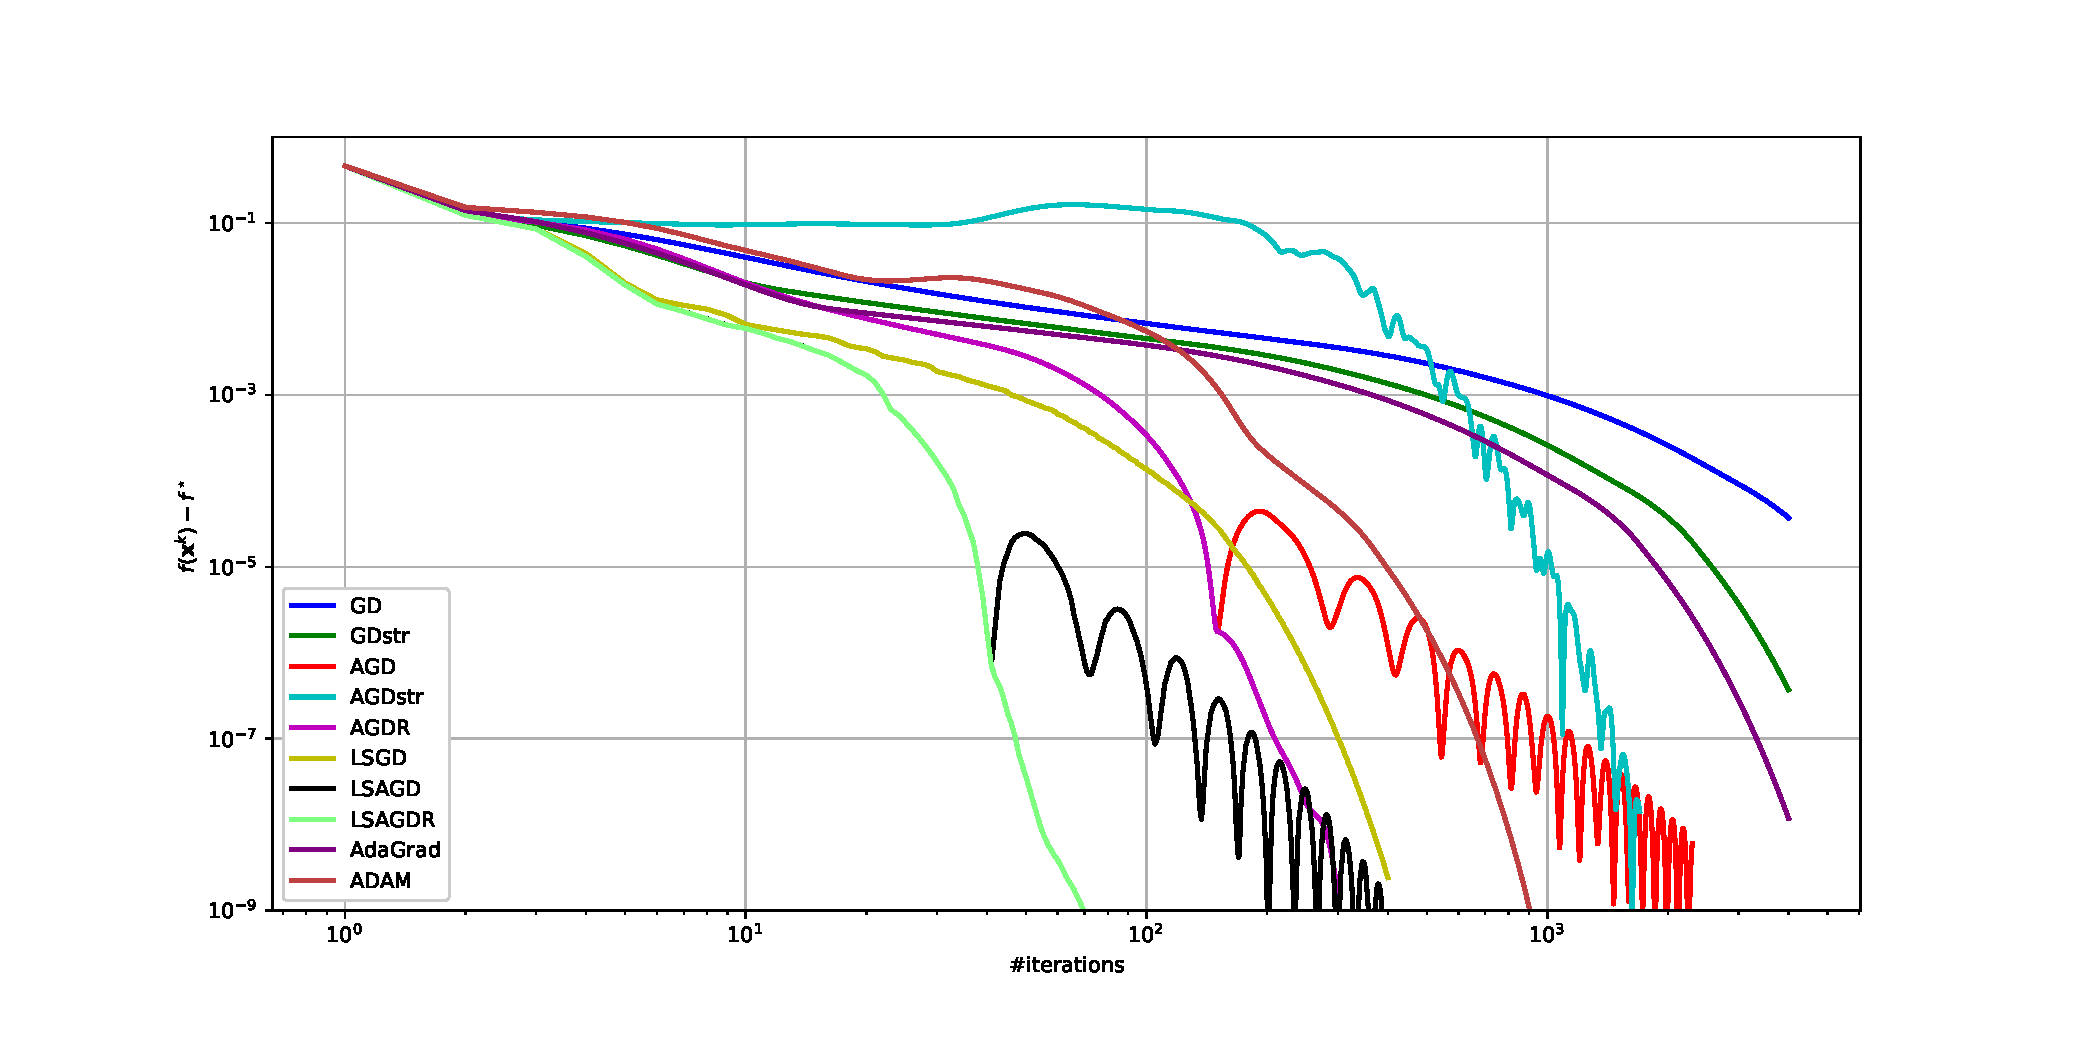
\includegraphics[scale=0.4]{2_iterations}
    \caption{Comparison in number of iterations for deterministic first-order methods}
    \label{fig:2_iterations}
\end{figure}
\begin{figure}[ht]
    \centering
    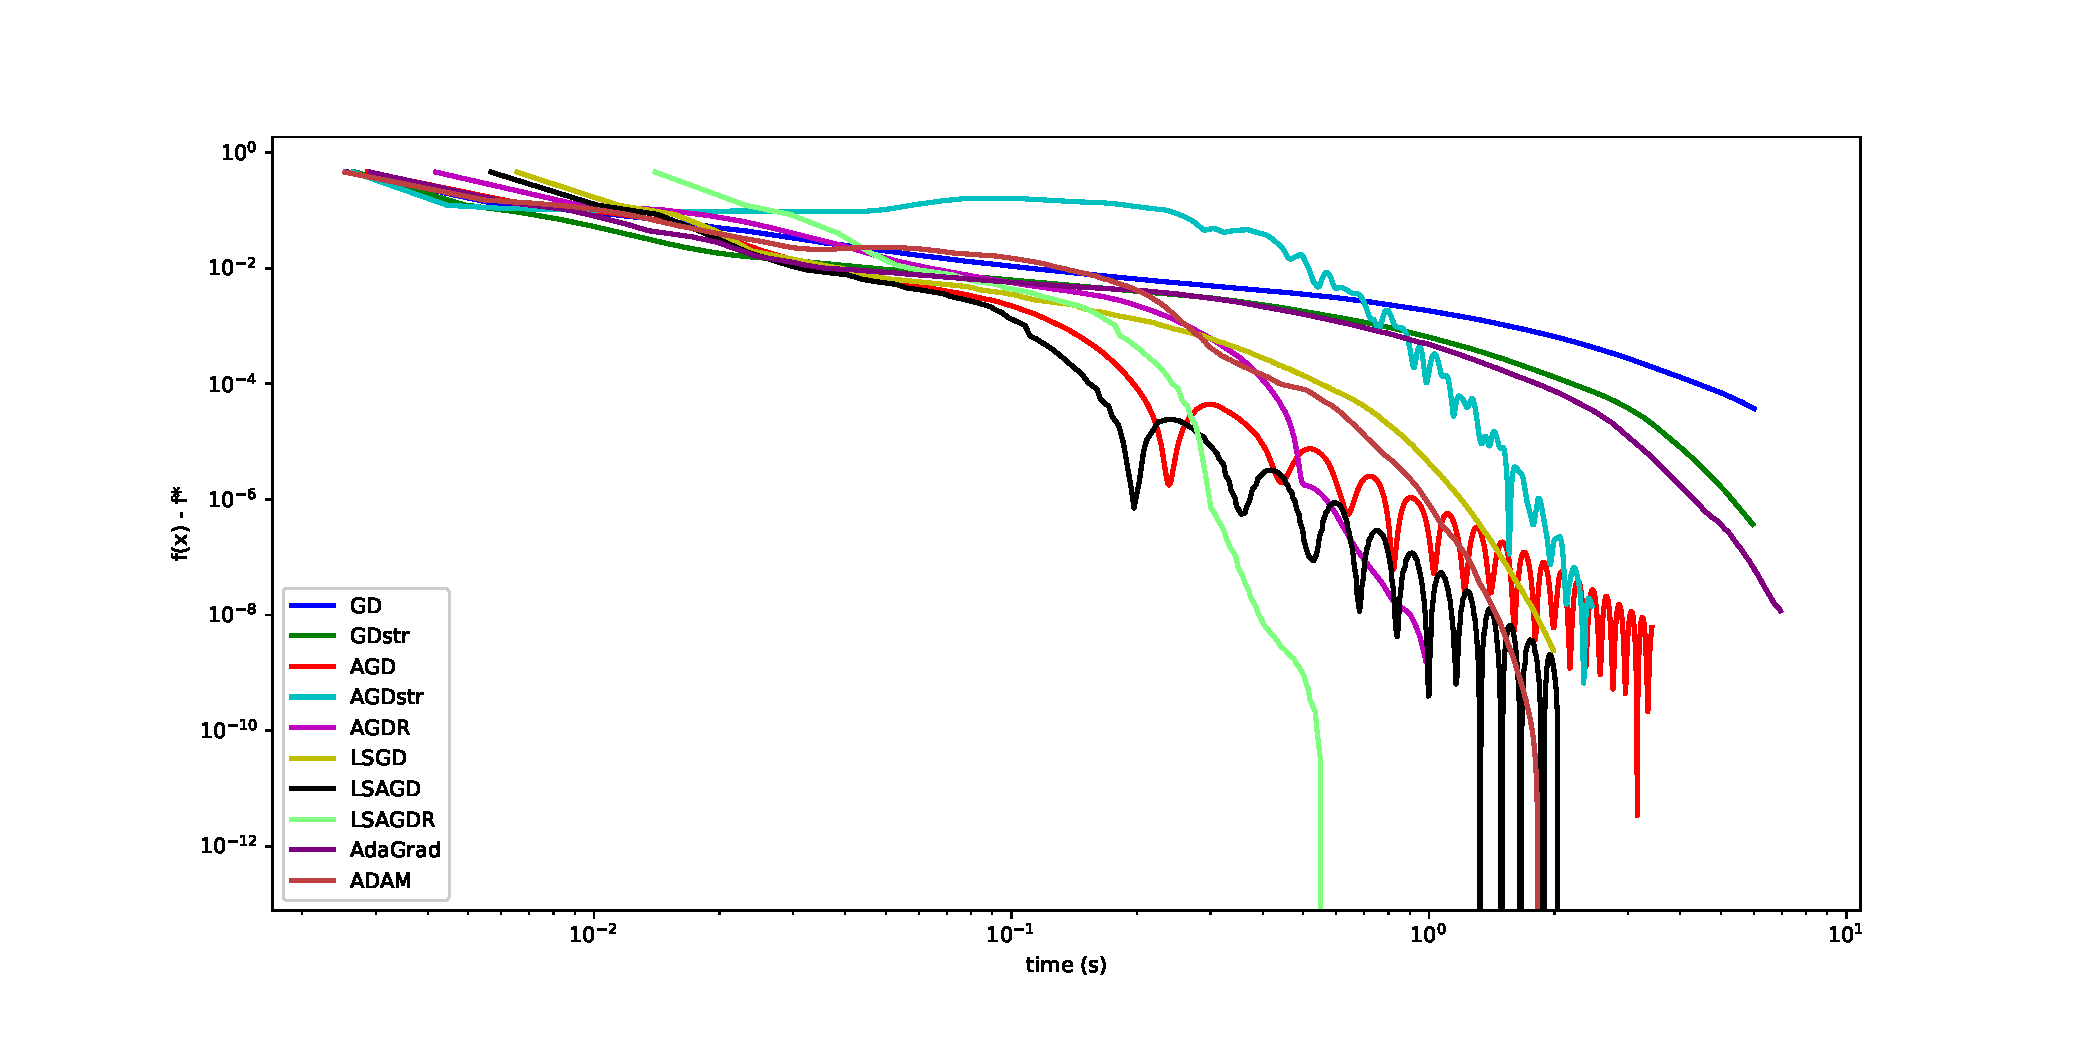
\includegraphics[scale=0.4]{2_time}
    \caption{Comparison in time for deterministic first-order methods}
    \label{fig:2_time}
\end{figure}

\begin{enumerate}[label=(\alph*)]
    \item \textbf{GD and GDstr: }As already expected, the gradient descent considering both the strong convexity of the function to optimize and its smoothness converges faster than that only considering smoothness (see Figure \ref{fig:2_iterations}). Moreover, the cost of each iteration is exactly the same since we are doing the same number of computations but only changing the learning rate. This can be seen in Figure \ref{fig:2_time}.
    
    \item \textbf{AGD and AGDstr: }Unlike the previous case, the Accelerated Gradient Descent algorithm works worse when we use information about the strong convexity of the function. Moreover, the cost per iteration is essentially the same as in the previous case, so this algorithms beat naive gradient descent in both number of iterations and time to converge.
    
    \item \textbf{LSGD and LAGD: }We converge with less iterations when we use the previous procedures with a step size that takes into account the local geometry. This step size is found by a linear search procedure, which translates into more cost (and thus more time) per iteration. Nevertheless, in this case we can see that the overhead is not significant enough for the previous algorithms to beat this version at almost any time.
    
    \item \textbf{AGDR and LAGDR: }The drawback of accelerated methods are that they are not monotone. In fact we can see the so-called Nesterov Ripples (oscillations) caused by the high momentum term, which is restarted in the algorithms presented in this section every time we increase the cost after one accelerated gradient step.
    
    For this reason, each of these algorithms is exactly the same as their non-restart version until the first oscillation as seen in Figure \ref{fig:2_iterations}. By construction, the restart version is now monotonic and thus the objective value decreases much faster than with the non-restart version.
    
    Nevertheless, note that iterations are slightly more costly with the restart version, specially when we actually restart since we compute two gradient steps in this iteration. Hence, in Figure \ref{fig:2_time}, we don't see the non-restart and restart versions sticking together for the first iterations as in Figure \ref{fig:2_iterations}.
    
    \item \textbf{AdaGrad: }This algorithm adapts to the local geometry of the problem with first-order information and doesn't need the Lipschitz constant as all the previous algorithms do nor the strong convexity constant as SGDstr and AGDstr. As seen in Figures \ref{fig:2_iterations} and \ref{fig:2_iterations}, this algorithm converges faster than Gradient Descent both in the number of iterations and in time, even if Gradient Descent uses an step size that is optimized for the Lipschitz and strong convexity constants of the function to optimize. Moreover, this algorithm introduces two new hyper-parameters, whose tuning sometimes could make a big difference.
    
    \item \textbf{ADAM: }Even if this algorithms can fail to converge to the global minimum of a convex problem, it usually performs well. Indeed in this case it converges faster that the previous adaptive algorithm and even faster than AGD knowing the Lipschitz constant. ADAM introduces four new hyper-parameters and thus depending on the time that we have to tune them or the performance in some problem with them taking the usual values, we may prefer other algorithms even if ADAM could achieve better results with the right tuning.
\end{enumerate}

\subsection*{Problem 3 - Stochastic Gradient methods for SVM}
\begin{enumerate}[label=(\alph*)]
    \item
    Since we choose each index $i_k$ uniformly at random from all the $n$ samples, we have that
    \begin{align}
        \E[\nabla f_{i_k}(\xx)] &= \frac{1}{n} \sum_{i=1}^{n} \nabla f_i(\xx) \\
        &= \lambda \xx + \frac{1}{n}\sum_{i=1}^n \left[ -b_i \aa_i\mathbbm{1}_{\{b_i \aa_i^T \xx  \leq 0\}} + \aa _i(\aa_i^T \xx - b_i )\mathbbm{1}_{\{0<b_i \aa_i^T \xx\leq 1\}} \right] \\
        &:= \nabla f(\xx)
    \end{align}
    where the last equality is the one already found in \eqref{eq:1}.
    
    \begin{assumption}
        Sample $i_k$ lies in the quadratic region
        \label{as:1}
    \end{assumption}
    
    Taking Assumption \ref{as:1}, we have that
    \begin{align}
        \norm{\nabla f_{i_k}(\xx) - \nabla f_{i_k}(\yy)} = \norm{\lambda(\xx - \yy) + \aa_{i_k} \aa_{i_k}^T (\xx - \yy)} \leq \norm{\lambda\mathbb{I} + \aa_{i_k} \aa_{i_k}^T}\norm{\xx + \yy}
    \end{align}
    where the inequality follows by definition of the spectral norm.
    
    Using triangle inequality as in problem 1 gives
    \begin{align}
        \norm{\lambda\mathbb{I} + \aa_{i_k} \aa_{i_k}^T} &\leq \lambda + \norm{\aa_{i_k} \aa_{i_k}^T} := \lambda + \max_{\xx:\norm{\xx}=1} \norm{\aa_{i_k} \aa_{i_k}^T x} := \lambda + \max_{\xx:\norm{\xx}=1} \sqrt{x^T \aa_{i_k} \aa_{i_k} ^T \aa_{i_k} \aa_{i_k}^T x} \\
        &:=\lambda + \max_{\xx:\norm{\xx}=1} \sqrt{x^T \norm{\aa_{i_k}} ^2 \norm{\aa_{i_k}} ^2 x} = \lambda + \norm{\aa_{i_k}} ^2 \max_{\xx:\norm{\xx}=1} \norm{x} = \lambda + \norm{\aa_{i_k}} ^2
    \end{align}
    
    Note that assumption \ref{as:1} is w.l.o.g. since if we lie on the linear region,
    \begin{align}
        \norm{\nabla f_{i_k}(\xx) - \nabla f_{i_k}(\yy)} = \norm{\lambda(\xx - \yy)} = \lambda \norm{\xx-\yy} < L\norm{\xx-\yy}
    \end{align}
    hence global smoothness is the same (valid upper bound) even if it's not locally tight for the samples in the linear region.
    
    \begin{figure}[ht]
        \centering
        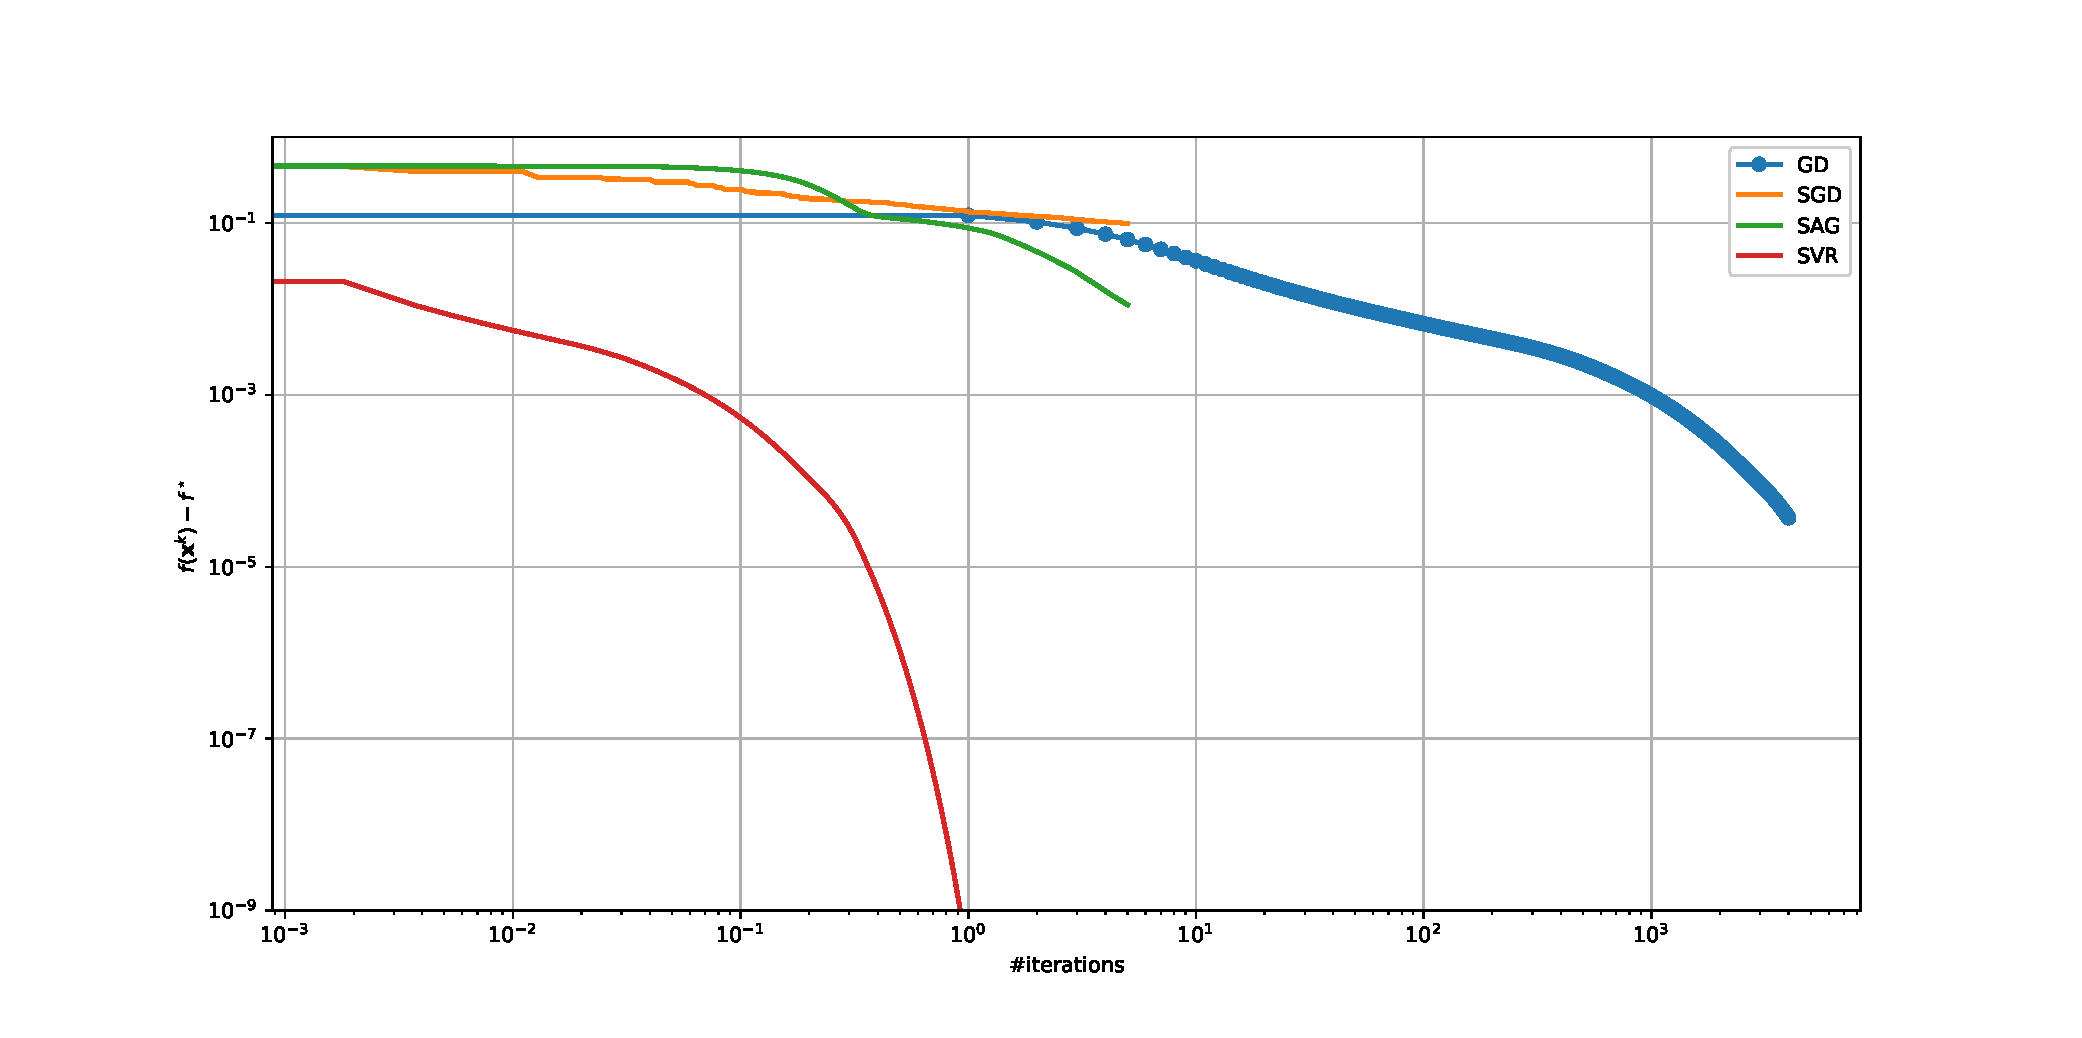
\includegraphics[scale=0.4]{3_iterations}
        \caption{Comparison in number of iterations for stochastic first-order methods}
        \label{fig:3_iterations}
    \end{figure}
    \begin{figure}[ht]
        \centering
        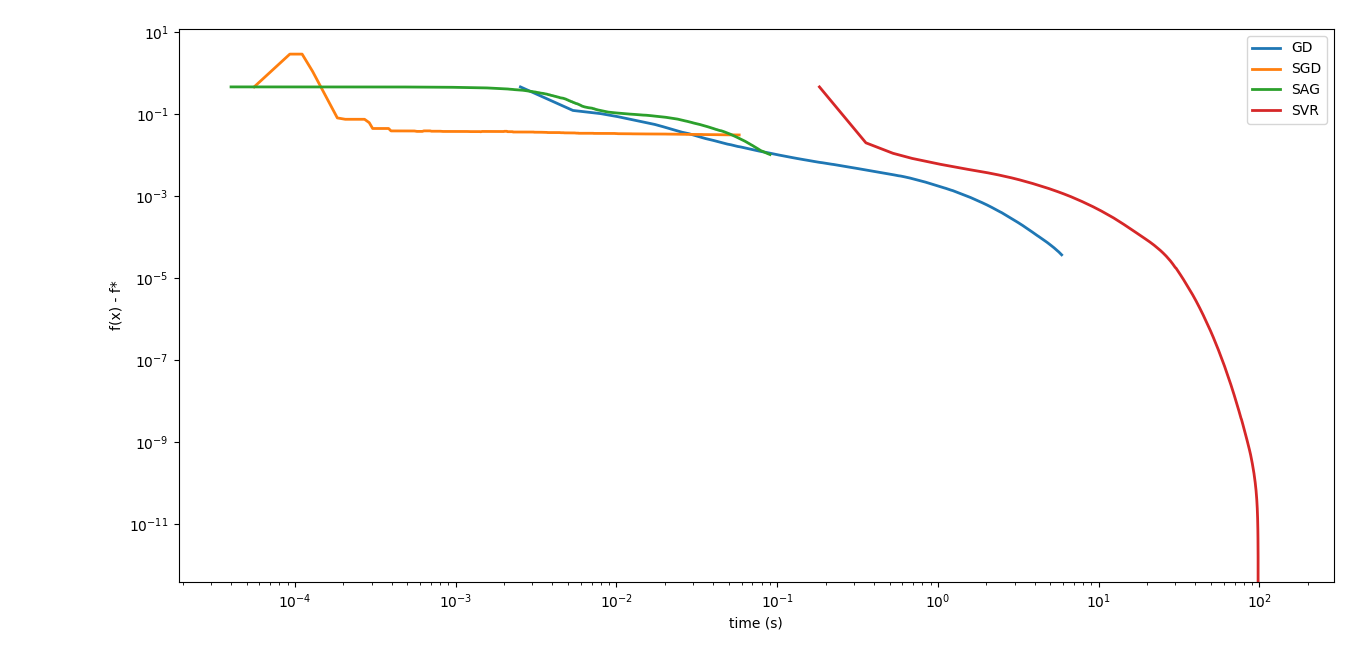
\includegraphics[scale=0.4]{3_time}
        \caption{Comparison in time for stochastic first-order methods}
        \label{fig:3_time}
    \end{figure}
    
    \item \textbf{SGD: }This algorithm has become the workhorse for training supervised machine learning problems which have a sum-structured objective function since the cost per iteration can be up to $n$ times cheaper than that of GD, where $n$ is the number of samples. When comparing to GD with respect to the number of iterations (Figure \ref{fig:3_iterations}), we see that the SGD requires a lot more iterations to converge since at each iteration we are only considering one random sample instead of the whole data as GD does. Nevertheless, the turns change when we compare these algorithms in time. As seen in Figure \ref{fig:3_time}, before GD performs the first iteration, SGD has achieved an objective value that can be good enough for some applications or even be used prior to methods that need a close start such as Newton's.
    
    \item \textbf{SAG: }When averaging stochastic gradients, we eventually get something similar to Gradient Descent if the variation of each gradient from one iteration to another is tiny (which happens near to a minimum). Thus, we can see that in comparison to SGD, we get better performance for the last iterations with exactly the same cost per iteration.
    
    \item \textbf{SVR: }This algorithm is the one that performs the best among all the ones seen before with respect to the number of iterations, since it essentially converges in only one iteration. Nevertheless, the variance reduction incurs an overhead at each iteration, making its cost $\mathcal{O}(1000L_{\max})$ times that of SGD. For this reason, we can see in Figure \ref{fig:3_time} that when SVR performs the first iteration, SGD has already done more than 2500 iterations.
    
\end{enumerate}

\end{document}
